\documentclass[12pt]{article}
\usepackage{amssymb, amsmath, amsfonts, bm, graphicx, geometry,cancel}
\usepackage{tabularx, booktabs, float, enumitem, multicol, mathtools}
\geometry{margin=1in}


\title{}
\date{}
\author{}
\DeclareMathOperator{\Real}{Re}
\DeclareMathOperator{\Imag}{Im}
\begin{document}

{\centering\LARGE Circuits Reference Sheet (Full)\par}\noindent
\section*{Units and SI Prefixes}
\makeatletter
\@fleqnfalse
\makeatother
\[\begin{aligned}
\text{femto (f)}  &= 10^{-15} \\
\text{pico (p)}   &= 10^{-12} \\
\text{nano (n)}   &= 10^{-9} \\
\text{micro ($\mu$)}  &= 10^{-6} \\
\text{milli (m)}  &= 10^{-3} \\
\text{centi (c)}  &= 10^{-2} \\
\text{deci (d)}   &= 10^{-1} \\
\text{deca (da)}  &= 10^{1} \\
\text{hecto (h)}  &= 10^{2} \\
\text{kilo (k)}   &= 10^{3} \\
\text{mega (M)}   &= 10^{6} \\
\text{giga (G)}   &= 10^{9} \\
\text{tera (T)}   &= 10^{12} \\
\text{peta (P)}   &= 10^{15} \\
\end{aligned}\]
\makeatletter
\@fleqntrue
\makeatother
\[1 e = 1.602 \times 10^{-19} \text{ C}\]
\newpage
\section*{Energy}
Energy storage: 1 J = 1 $\text{W}\cdot\text{s}$, 1 Wh = 3600 J
\[W = \int P\,dt = \int VI\, dt = VQ\quad \text{or} \quad P\Delta t \text{ (constant power)}\]
Units:
\begin{itemize}
    \item $W$: energy in [J] or [Wh]
    \item $P$: power in [W]
    \item $V$: voltage in [V] or [J/C]
    \item $I$: current in [A] or [C/s]
    \item $Q$: charge capacity in [C] or [Ah]
\end{itemize}
Ex: Battery capacity\\\\
Battery life: 
\[t=\frac{W}{P}\quad \frac{[\text{Wh}]}{[\text{W}]}\]
Charge time:
\[t=\frac{Q}{I_\text{eff}}\quad \frac{[\text{Ah}]}{[\text{A}]}, \quad I_\text{eff} = I_\text{in}\cdot \eta\]
\section*{Power}
Power: $P = VI = I^2R = \frac{V^2}{R}$
\section*{Resistance}
Resistance: $R = \rho \frac{L}{A}\quad [\Omega]$
\section*{Conductance}
Conductance: $G = \frac{1}{R}=\sigma \frac{A}{L}\quad [\text{S}]$
\section*{Resistors in Series and Parallel}
Series: 
\[R_\text{eq} = R_1 + R_2 + \cdots + R_n\]
Parallel: 
\[\frac{1}{R_\text{eq}} = \frac{1}{R_1} + \frac{1}{R_2} + \cdots + \frac{1}{R_n}\]
\[\implies R_\text{eq} - \frac{R_1R_2}{R_1+R_2}\]
\section*{*Combining Sources}
Voltage sources in \underline{series} add
\begin{center}
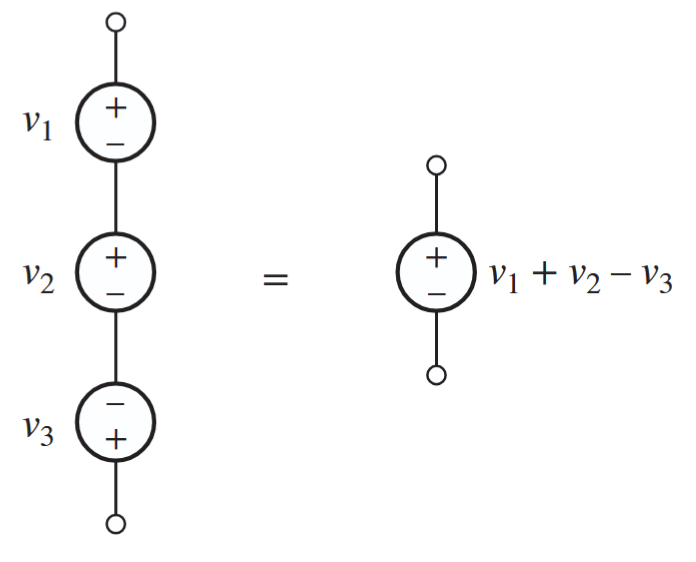
\includegraphics[width=0.5\textwidth]{../../Series V.png}
\end{center}
Current sources in \underline{parallel} add
\begin{center}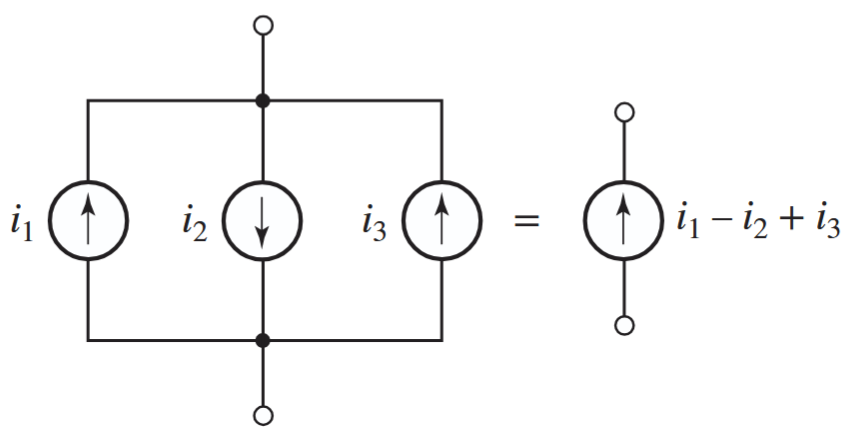
\includegraphics[width=0.5\textwidth]{../../Parallel C.png}
\end{center}
\section*{*Source Transformations}
\begin{center}
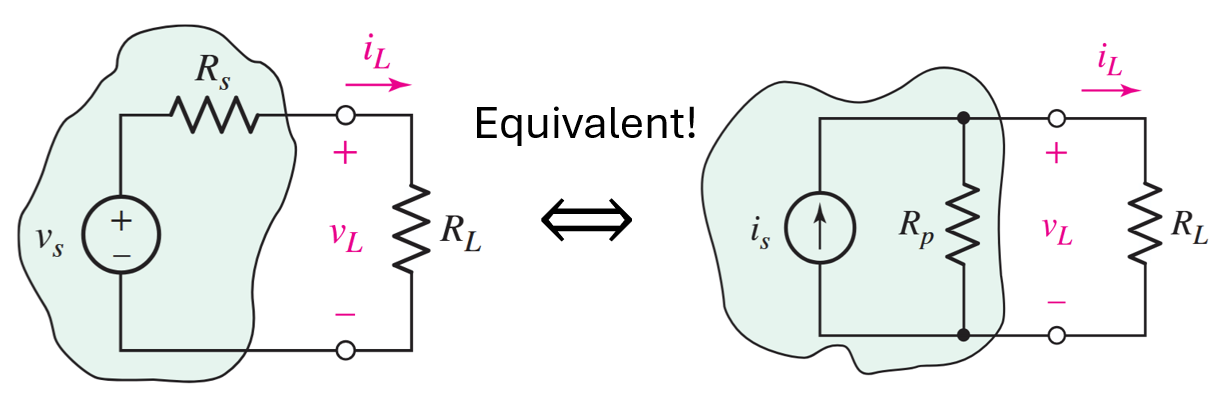
\includegraphics[width=0.8\textwidth]{../../Source Transformation.png}
\end{center}
The circuits above are equivalent if
\[R_s = R_p \quad\text{AND}\quad V_s=i_sR_s\]
\section*{Nodal Analysis (KCL)}
\[I_{R_1} = \frac{V_1-V_2}{R_1}\quad \text{(voltage drop in the direction of current flow)}\]
\textbf{Supernode:} Around \textit{voltage source} ($V_3-V_4=V_\text{source}$)
\section*{Mesh Analysis (KVL)}
\[V_{R_1} = I_{R_1}R_1\]
\textbf{Supermesh:} Loop around \textit{current source} ($i_1 - i_2 = i_\text{source}$)
\section*{Voltage Division in Series}
\[V_k = \frac{R_k}{R_1 + R_2 + \cdots + R_n} V_\text{source}\]
\section*{Current Division in Parallel}
\[I_k = \frac{\frac{1}{R_k}}{\frac{1}{R_1} + \frac{1}{R_2} + \cdots + \frac{1}{R_n}} I_\text{source}\]
\section*{Superposition}
Isolate each source, turn off all other source (voltage sources become short circuit, current sources become open circuit). Solve for circuit response from each source, then add responses together.
\[i_x = i_x'+ i_x'', \quad v_x = v_x'+ v_x''\]
\section*{Thevenin and Norton Equivalent Circuits}
\begin{itemize}
    \item Thevenin equivalent: Voltage source $V_{Th}$ in series with resistance $R_{Th}$
    \item Norton equivalent: Current source $i_{N}$ in parallel with resistor $R_{N}$
    \item They are source transformations of each other:
    \[ V_{Th} = i_N R_{Th}, \quad R_{Th} = R_N \]
\end{itemize}
\textbf{Finding the Equivalent Source}
\begin{itemize}
    \item $V_{Th}=V_{oc}$ (open circuit voltage): disconnect the load $R_L$ and solve for the voltage across the open terminals
    \item $i_{N}=i_{sc}$ (short circuit current): short the load (replace $R_L$ with a wire) and solve for the current flowing through the short
\end{itemize}
\textbf{Finding the equivalent resistance seen from the load $\mathbf{R_L}$}
\begin{itemize}
    \item \underline{If only independent sources:} turn off all independent sources (voltage = short/wire, current = open/break). Sum resistances in remaining circuit
    \item \underline{If dependent source:}
    \begin{itemize}
        \item Find the open circuit voltage and short circuit current as above, then calculate $R_{Th} = \frac{V_{oc}}{i_{sc}}$
        \item OR turn off independent sources, and apply a test voltage ($V_\text{test}$ or $1\text{V}$) and solve for the resulting current. Can also apply a test current ($I_\text{test}$ or $1\text{A}$) and solve for resulting voltage. Apply test voltage/current across the load terminals, and $R_\text{Th} = \frac{V_\text{test}}{I_\text{test}}$
    \end{itemize}
\end{itemize}
\textbf{Max power transfer condition:}
\[R_L = R_{Th}\]
\newpage
\section*{Operational Amplifiers}
\begin{itemize}
    \item \textbf{Inverting Amplifier}
    \begin{center}
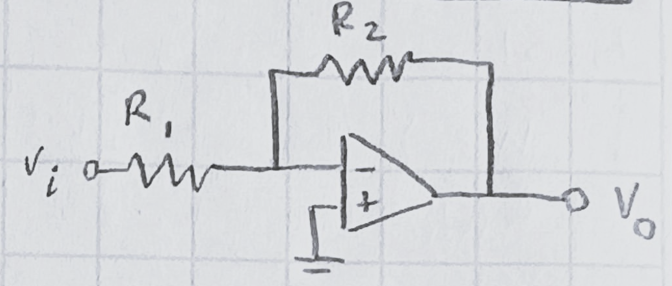
\includegraphics[width=0.4\textwidth]{inverting.png}
    \end{center}
    \[v_o=-\frac{R_2}{R_1}v_i\]
    \item \textbf{Non-inverting Amplifier}
    \begin{center}
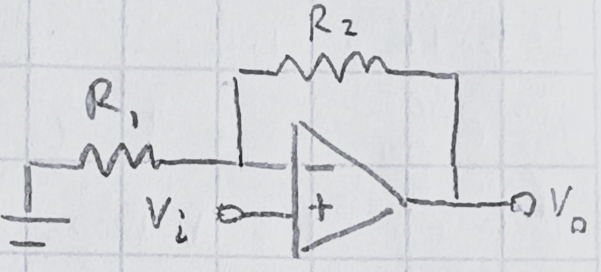
\includegraphics[width=0.4\textwidth]{noninverting.png}
    \end{center}
    \[v_o=\left(1+\frac{R_2}{R_1}\right)v_i\]
    \item \textbf{Buffer (Voltage Follower)}
    \begin{center}
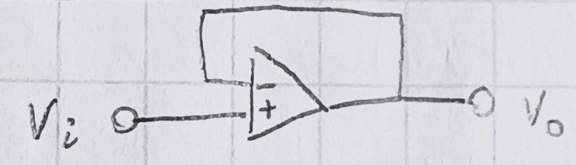
\includegraphics[width=0.4\textwidth]{buffer.png}
    \end{center}
    \[v_o=v_i\]
    \item \textbf{Summer}
    \begin{center}
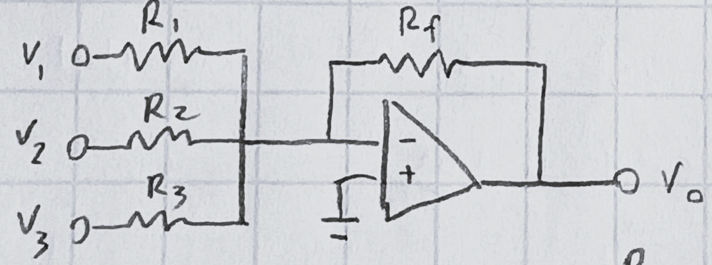
\includegraphics[width=0.4\textwidth]{summer.png}
    \end{center}
    \[v_o=-\left(\frac{R_f}{R_1}v_1+\frac{R_f}{R_2}v_2+\frac{R_f}{R_3}v_3\right)\]
    \newpage
    \item \textbf{Difference Amplifier}
    \begin{center}
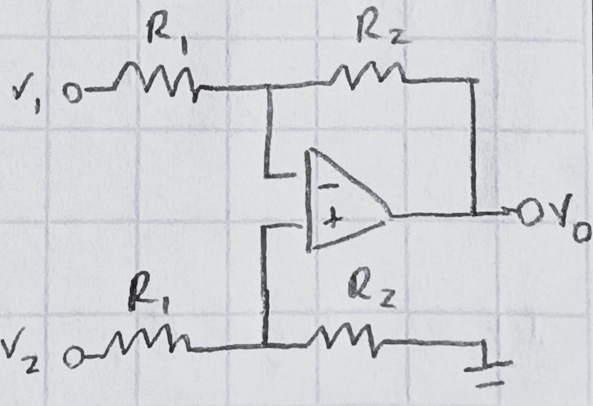
\includegraphics[width=0.4\textwidth]{difference.png}
    \end{center}
    \[v_o=\frac{R_2}{R_1}(v_2-v_1)\]
\end{itemize}
\section*{Energy Storage in Capacitors}
\textbf{Capacitance:}
\[C=\frac{\varepsilon_0\varepsilon_r A}{d}\quad \text{(parallel plate)}\]
Where $\varepsilon_0=8.854\times10^{-12} \text{ F/m}$ is the permittivity of free space\\\\
\textbf{Energy stored in a capacitor: }
\[w= \frac{1}{2}CV^2 = \frac{q^2}{2C}\]
\textbf{Summing capacitors in series and parallel:}
\begin{itemize}
    \item Series: $\frac{1}{C_\text{eq}} = \frac{1}{C_1} + \frac{1}{C_2} + \cdots + \frac{1}{C_n}$
    \item Parallel: $C_\text{eq} = C_1 + C_2 + \cdots + C_n$
\end{itemize}
\textbf{Properties of Capacitors}
\begin{itemize}
    \item A capacitor at steady state (DC) behaves like an open circuit
    \item \textit{Voltage across a capacitor must be continuous}: $v_C(0^+) = v_C(0^-)$
    \item \textit{Current through a capacitor can be discontinuous}: $i_C(0^+) \neq i_C(0^-)$
\end{itemize}
\section*{Energy Storage in Inductors}
\textbf{Inductance:}
\[L = \frac{N^2 \mu A}{l}\quad \text{(solenoid)}\]
Where $\mu = \mu_0 \mu_r$ is the permeability of the core material, and $\mu_0 = 4\pi \times 10^{-7} \text{ H/m}$ is the permeability of free space\\\\
\textbf{Energy stored in an inductor:}
\[w = \frac{1}{2}LI^2\]
\textbf{Summing inductors in series and parallel:}
\begin{itemize}
    \item Series: $L_\text{eq} = L_1 + L_2 + \cdots + L_n$
    \item Parallel: $\frac{1}{L_\text{eq}} = \frac{1}{L_1} + \frac{1}{L_2} + \cdots + \frac{1}{L_n}$
\end{itemize}
\textbf{Properties of Inductors}
\begin{itemize}
    \item An inductor at steady state (DC) behaves like a short circuit
    \item \textit{Current through an inductor must be continuous}: $i_L(0^+) = i_L(0^-)$
    \item \textit{Voltage across an inductor can be discontinuous}: $v_L(0^+) \neq v_L(0^-)$
\end{itemize}
\begin{table}[H]
\centering
\renewcommand{\arraystretch}{2}
\begin{tabular}{|c|c|c|c|}
\hline
\textbf{Relation} & \textbf{Resistor ($R$)} & \textbf{Capacitor ($C$)} & \textbf{Inductor ($L$)} \\
\hline

$v-i:$ &
$\displaystyle v=iR$ &
$\displaystyle v=\frac{1}{C}\int_{t_0}^{t} i(\tau)\,d\tau + v(t_0)$ &
$\displaystyle v=L\frac{di}{dt}$ \\
\hline

$i-v:$ &
$\displaystyle i=\frac{v}{R}$ &
$\displaystyle i=C\frac{dv}{dt}$ &
$\displaystyle i=\frac{1}{L}\int_{t_0}^{t} v(\tau)\,d\tau + i(t_0)$ \\
\hline

$P$ or $W:$ &
$\displaystyle p=i^2R=\frac{v^2}{R}$ &
$\displaystyle w=\frac{1}{2}Cv^2$ &
$\displaystyle w=\frac{1}{2}Li^2$ \\
\hline

Series &
$\displaystyle R_{eq}=R_1+R_2$ &
$\displaystyle C_{eq}=\frac{C_1C_2}{C_1+C_2}$ &
$\displaystyle L_{eq}=L_1+L_2$ \\
\hline

Parallel &
$\displaystyle R_{eq}=\frac{R_1R_2}{R_1+R_2}$ &
$\displaystyle C_{eq}=C_1+C_2$ &
$\displaystyle L_{eq}=\frac{L_1L_2}{L_1+L_2}$ \\
\hline

At DC: &
Same &
Open circuit &
Short circuit \\
\hline

\begin{tabular}[c]{@{}c@{}}
Circuit variable \\
that cannot \\
change abruptly:
\end{tabular}
&
Not applicable &
$v$ &
$i$ \\
\hline

\end{tabular}
\end{table}
\section*{Operational Amplifiers with Energy Storage}
\begin{itemize}
    \item \textbf{Integrator}
    \begin{center}
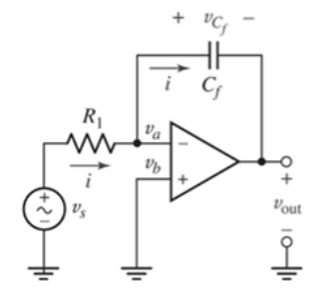
\includegraphics[width=0.4\textwidth]{integrator.png}
    \end{center}
    \[v_o = -\frac{1}{R_1C_f}\int_0^t v_s(t')\,dt'-v_{C_f}(0)\]
    \item \textbf{Differentiator}
    \begin{center}
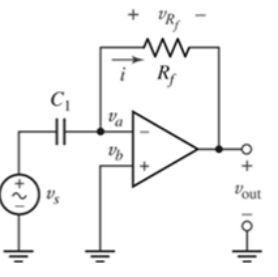
\includegraphics[width=0.4\textwidth]{differentiator.png}
    \end{center}
    \[v_o = -C_1R_f\frac{dv_s}{dt}\]
\end{itemize}
\newpage
\section*{First Order RC and RL Circuit Responses (DC)}
\textbf{Driven RC Circuit Step Response}
\begin{enumerate}
    \item With all independent sources zeroed out, simplify the circuit to determine $R_{\text{eq}}$ and $C_{\text{eq}}$, and the time constant $\tau_{\text{eq}} = R_{\text{eq}} C_{\text{eq}}$.
    \item Determine the initial condition $v(0^+)$ or $i(0^+)$ [recall that the capacitor voltage is continuous: $v_c(0^-) = v_c(0^+)$]
    \item Determine the steady state condition $v(\infty)$ or $i(\infty)$.
    \item The final response is given by:
  \[\boxed{\begin{aligned}
    v(t) &= v(\infty) + [v(0^+) - v(\infty)] e^{-t/\tau_{\text{eq}}} \\
    i(t) &= i(\infty) + [i(0^+) - i(\infty)] e^{-t/\tau_{\text{eq}}}
    \end{aligned}}\]
\end{enumerate}
\textbf{Driven RL Circuit Step Response}
\begin{enumerate}
    \item With all independent sources zeroed out, simplify the circuit to determine $R_{\text{eq}}$ and $L_{\text{eq}}$, and the time constant $\tau_{\text{eq}} = L_{\text{eq}}/R_{\text{eq}}$.
    \item Determine the initial condition $v(0^+)$ or $i(0^+)$ [recall the requirement that any inductor current $i_L(0^-) = i_L(0^+)$].
    \item Determine the final condition $v(\infty)$ or $i(\infty)$.
    \item The final response is given by
     \[\boxed{\begin{aligned}
    v(t) &= v(\infty) + [v(0^+) - v(\infty)] e^{-t/\tau_{\text{eq}}} \\
    i(t) &= i(\infty) + [i(0^+) - i(\infty)] e^{-t/\tau_{\text{eq}}}
    \end{aligned}}\]
\end{enumerate}
\underline{Note:} For a \textit{natural response} (no forcing function), the steps above still apply, but the steady state values go to zero: $v(\infty) = 0$ and $i(\infty) = 0$.
\section*{Second Order RLC Circuit Responses (DC)}
\textbf{Defining Frequencies and Damping}
For a RLC circuit:
\begin{itemize}
    \item Natural Frequency: $\omega_0 = \frac{1}{\sqrt{LC}}$
    \item Exponential damping coefficient: $\alpha = \frac{1}{2RC}\quad \text{(parallel RLC)}$, $\alpha = \frac{R}{2L}\quad \text{(series RLC)}$
    \item Damping Ratio: $\zeta = \alpha/\omega_0$
\end{itemize}
\underline{Note:} Overdamped: $\zeta > 1$, Critically damped: $\zeta = 1$, Underdamped: $\zeta < 1$.\\\\
\textbf{Solving for the Time Domain Response:}
\begin{table}[H]
\centering
\begin{tabular}{lll}
\hline
\textbf{Response Type} & \textbf{Condition} & \textbf{General Solution (for both $i(t)$ and $v(t)$)} \\ \hline
& & \\
\textbf{Overdamped} & $\alpha > \omega_0$ & $i(t) = A_1e^{s_1t} + A_2e^{s_2t}$ \\
& & \\ \hline
& & \\
\textbf{Critically Damped} & $\alpha = \omega_0$ & $i(t) = e^{-\alpha t}(A_1t + A_2)$ \\
& & \\ \hline
& & \\
\textbf{Underdamped} & $\alpha < \omega_0$ & $i(t) = e^{-\alpha t}(B_1 \cos \omega_d t + B_2 \sin \omega_d t),\quad \omega_d = \sqrt{\omega_0^2 - \alpha^2}$ \\
& & \\ \hline
\end{tabular}
\end{table}
\noindent
\underline{Note:} The exponents $s_1$ and $s_2$ are simply $-\alpha \pm \sqrt{\alpha^2 - \omega_0^2}$. Solve for the constants $A_1$, $A_2$, $B_1$, and $B_2$ using the initial conditions of the problem.\\\\
In the case of a DRIVEN RLC circuit, the total response is the sum of the natural response and the forced response (steady state value for $i$ or $v$).
\section*{Second Order RLC Circuit Responses (Sinusoidal Steady State)}
\begin{itemize}
    \item A sinusoidal forcing function always results in a sinusoidal forced response of the same frequency in a linear circuit. This means that if the input is a sine then the output is a sine of the same frequency, but possibly different amplitude and phase. 
    \item We can rewrite sinusoidal functions as the real and imaginary part of a complex exponential through Euler's identity
    \[e^{j\omega t} = \cos(\omega t) + j\sin(\omega t)\]
    \[cos(\omega t + \phi) = \Real\{e^{j(\omega t + \phi)}\}\]
    \[\sin(\omega t + \theta) = \Imag\{e^{j(\omega t + \theta)}\}\]
    \item Since all sinusoidal functions have the same frequency, we can use phasor notation, supressing the time dependence term $e^{j\omega t}$, resulting in a phasor.
   \begin{center}
    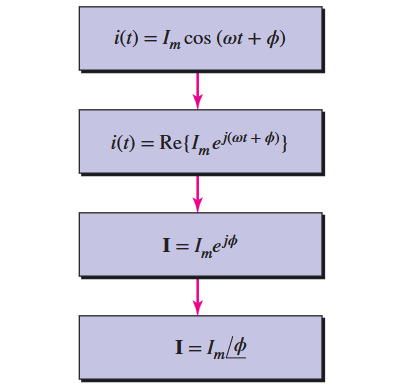
\includegraphics[width=0.4\textwidth]{../HW8/Phasor transform.png}
   \end{center}
   Note that $\mathbf{I}$ represent complex numbers, and we will take the real or imaginary part of the resulting phasor to get to the actual time domain response.\\\\
   Additionally, differentiation and integration in the time domain correspond to multiplication and division by $j\omega$ in the phasor domain, respectively.
   \item $\mathbf{V}$ and $\mathbf{I}$ relationships:
   \begin{center}
    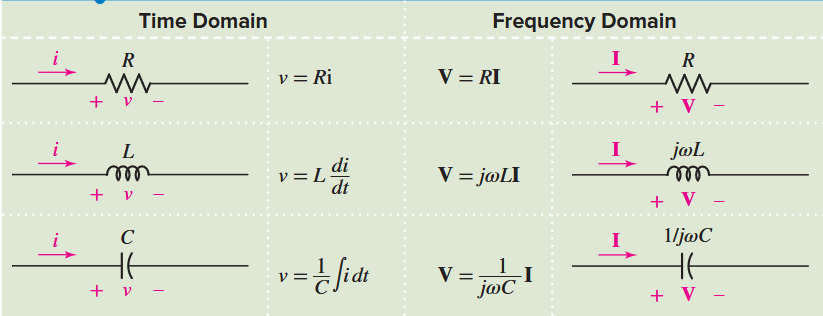
\includegraphics[width=0.8\textwidth]{../HW8/VI.png}
   \end{center}
   We can use these complex valued currents and voltages with KCL and KVL as we normally would to analyze circuits, and then take the real or imaginary part of the resulting phasor to get to the actual time domain response.
   \item We define \textbf{impedance} to be the relationship between the complex voltage and current in a circuit element:
   \[\mathbf{Z} = \frac{\mathbf{V}}{\mathbf{I}}\]
   These impedances sum in series and parallel just like resistances and can also be used in nodal and mesh analysis using the relationship $\mathbf{V} = \mathbf{IZ}$ (just like Ohm's law).
   \item Since $\mathbf{Z}$ is a complex number, we can express it either in rectangular form $\mathbf{Z} = R + jX$ or in polar form $\mathbf{Z} = |\mathbf{Z}|e^{j\theta}$, where $R$ is the real part of the impedance (resistance), and $X$ is the imaginary part of the impedance (reactance).  
   \item Although we have complex voltages and currents for sinusoidal sources, because the circuit is linear, \textbf{superposition}, \textbf{source transformations}, and \textbf{Thevenin/Norton equivalents} still apply in the phasor domain. Just remember to use impedances instead of resistances.
\end{itemize}
\section*{Coupled Coils}
\begin{itemize}
    \item \textbf{Dot Convention for Mutual Inductance}:
    \begin{itemize}
        \item A current entering the \textit{dotted} terminal of one coil produces an open-circuit voltage with a positive voltage reference at the \textit{dotted} terminal of the second coil.
        \item A current entering the \textit{undotted} terminal of one coil provides a voltage that is positively sensed at the \textit{undotted} terminal of the second coil
    \end{itemize}
    \begin{center}
        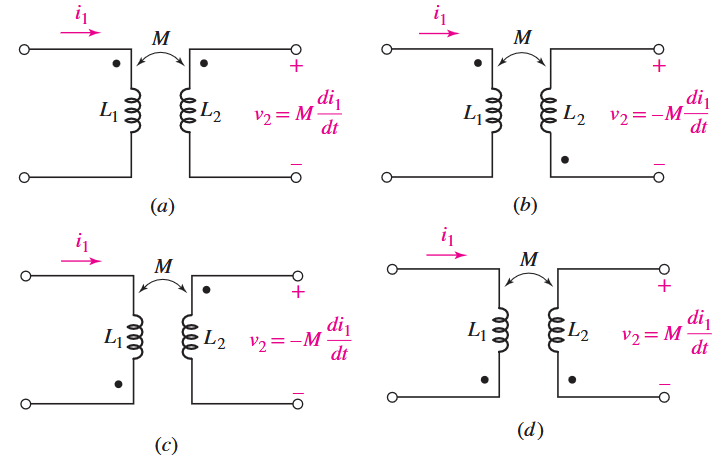
\includegraphics[width=0.8\textwidth]{../HW9/dot.png}
    \end{center}
    Note that \textbf{self-induction} exists if the current in the right loop ($i_2$) is non-zero and would cause back emf.
    \item Total energy in coupled inductors:
    \begin{center}
        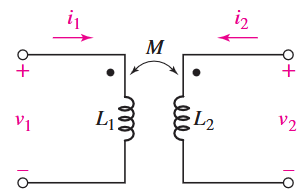
\includegraphics[width=0.4\textwidth]{../HW9/energy.png}
    \end{center}
    \[w(t)=\frac{1}{2}L_1[i_1(t)]^2 + \frac{1}{2}L_2[i_2(t)]^2 + M[i_1(t)][i_2(t)]\]
    \textbf{Limit on M}:
    \[M \leq \sqrt{L_1 L_2}\]
    \textbf{Coupling coefficient:}
    \[k = \frac{M}{\sqrt{L_1 L_2}} \implies 0 \leq k \leq 1\]
    \item Linear transformer and reflected impedance:
    \begin{center}
        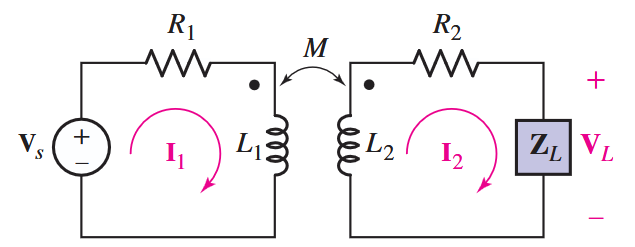
\includegraphics[width=0.6\textwidth]{../HW9/transformer.png}
    \end{center}
    The \textit{primary circuit} contains the source $v_s$ and the \textit{secondary circuit} contains the load $\mathbf{V_L}$.\\\\
    By using mesh analysis on each of the two loops, we can simplify the circuit to an equivalent circuit with a $\mathbf{V_s}$ in series with a reflected impedance $\mathbf{Z_\text{in}}$:
    \[\frac{\mathbf{V_s}}{\mathbf{I_1}} = \mathbf{Z_\text{in}} = \mathbf{Z_{11}}-\frac{(j\omega)^2M^2}{\mathbf{Z_{22}}}\]
    Where $\mathbf{Z_{11}}$ and $\mathbf{Z_{22}}$ are the self-impedances of the primary and secondary circuits, respectively. 
    \[\mathbf{Z_{11}} = R_1+j\omega L_1\]
    \[\mathbf{Z_{22}} = R_2+j\omega L_2 + \mathbf{Z_L}\]
    \item \textbf{Ideal Transformer}:
    \begin{center}
        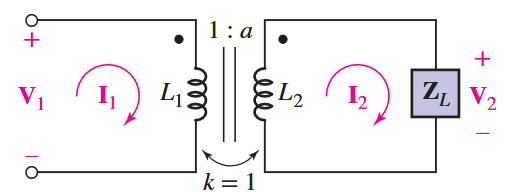
\includegraphics[width=0.6\textwidth]{../HW9/ideal.png}
    \end{center}
    In an ideal transformer, the coupling coefficient $k=1$ and the mutual inductance $M = \sqrt{L_1 L_2}$.\\\\
    \textbf{Turns Ratio:}
    \[a^2 = \frac{L_2}{L_1} = \frac{N_2^2}{N_1^2}\]
    Using turns ratio, we can have the following relationships:
    \[\frac{1}{a} = \frac{I_2}{I_1}\]
    \[a = \frac{V_2}{V_1}\]
    \[a^2 = \frac{\mathbf{Z_L}}{\mathbf{Z_\text{in}}}\]
\end{itemize}









\end{document}